Для реализации поставленной задачи исследования в магистерской
диссертации был выбран пакет моделирования процессов столкновения элементарных частиц при высоких энергиях на ускорителях элементарных частиц \textit{PYTHIA} на языке программирования \textit{С++}, а также принято решение о реализации всего программного
комплекса на языке программирования \textit{Java}.
В качестве веб интерфейса был использован фреймворк \textit{Angular} на языке программирования \textit{JavaScript}. Так же была использована и бибилотека \textit{d3js} для отрисовки графиков в виде \textit{SVG} изображений и взаимодействия пользователя с интерфейсом приложения.

Когда говорят о научных основах проектирования пользовательских
интерфейсов, в первую очередь упоминают термин \textit{Human-Computer Interaction}
(\textit{HCI}) – «взаимодействие человека и компьютера». В странах Запада \textit{HCI} это
является целой профессией, ей обучают в университетах, издается много
журналов по этой теме, существует большое количество \textit{web}-сайтов~\cite{user-interface}.
Составными частями \textit{HCI} являются:

\begin{enumerate}
	\item[--] человек (пользователь);
	\item[--] компьютер;
	\item[--] их взаимодействие.
\end{enumerate}

Пользовательский интерфейс \textit{user interface} (\textit{UI}) – является своеобразным
коммуникационным каналом, по которому осуществляется взаимодействие
пользователя и компьютера.

Лучший пользовательский интерфейс – это такой интерфейс, которому
пользователь не должен уделять много внимания, почти не замечать его. В руках
пользователя интерфейс пользователя должен служить инструментом для
достижения цели. Такой интерфейс называют прозрачным – пользователь
смотрит сквозь него на свою работу.

Чтобы создать эффективный интерфейс, который делал бы работу с
программным комплексом эффективной, нужно понимать, какие задачи будут
решать пользователи с помощью данной программного комплекса и какие
требования к интерфейсу могут возникнуть у пользователей. Большую роль в
разработке интерфейса играет интуиция – если разработчик сам терпеть не
может некрасивые и неудобные интерфейсы, то при создании собственного
программного комплекса он будет чувствовать, где и какой именно элемент
нужно убрать или добавить. Необходимо иметь художественный вкус, чтобы
понимать, что именно придаст интерфейсу красоту и привлекательность.

Западные исследователи в области \textit{HCI} сформулировали основные
принципы проектирования пользовательских интерфейсов компьютерных
программ~\cite{user-interface}. Как и в любой другой отрасли ИТ, существует довольно много
различных методик и классификаций. Можно сформировать три положения
говоря об общих принципах проектирования пользовательского интерфейса:

\begin{enumerate}
	\item[--] программный комплекс должен помогать выполнить задачу, а не
	становиться этой задачей;
	\item[--] при работе с программой пользователь не должен думать, что он не
	понимает программу;

	\item[--] программный комплекс должен работать так, чтобы пользователь не
	считал компьютер бесполезным инструментом.
\end{enumerate}

Конечно, глубина проработки интерфейса и степень его адаптивности под
нужды пользователя в программных комплексах в основном зависит от усилий
их авторов, а не от характеристик аппаратного обеспечения. Однако у
большинства пользователей компьютер ассоциируется именно с программными
комплексами, которые на нем работают, и плохое впечатление от использования
программного обеспечения автоматически переносится на сам компьютер.

Открыв начальную веб-страницу приложения в любом из доступных браузеров пользователь увидит сообщение с описанием проекта, как показано на рисунке~\ref{fig:welcome-page}.

\begin{figure}[!h]
	\centering
	
\includegraphics[width=\textwidth]{figures/welcome-page.png}
	\caption{Начальная \textit{web}-страница}
	\label{fig:welcome-page}
\end{figure}

Сообщество разработчиков фреймворка \textit{Angular} разрабатывает дополнительные компоненты \textit{Angular Material Design} и предлагает использовать их для быстрой разработки приложения с нуля. 

\textit{Material Design} -- визуальный язык, представлен в 2014 году \textit{Google}, используется чаще всего в мобильных приложения. Пример использования \textit{Material Design} можно увидеть во многих мобильных приложения \textit{Google} (\textit{Play, Music, Books} и т.д.), а также в \textit{Chrome OS}. \textit{Material Design} упрощает разработчикам настройку \textit{UI}, сохраняя при этом удобный интерфейс приложений. \textit{Angular Material} состоит из набора предустановленных компонентов \textit{Angular}. \textit{Anglate Material} стремится обеспечить расширенный и последовательный пользовательский интерфейс. В то же время он дает возможность контролировать, как ведут себя разные компоненты.

Для каждого пользователя на начальной странице приложения располагается навигационное меню, котрое показано на рисунке~\ref{fig:menu}. Так как разработанное приложение является одностраничным то переход по пунктам меню не перезагружает страницу полностью, а лишь подгружает необходимые компоненты.

\begin{figure}[!h]
	\centering
	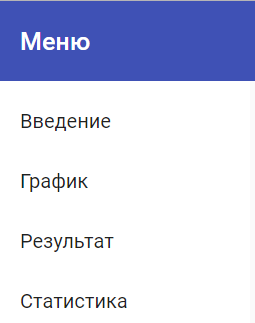
\includegraphics[width=0.5\textwidth]{figures/menu.png}
	\caption{Главное меню приложения}
	\label{fig:menu}
\end{figure}

Из главного меню доступен переход на следующие страницы приложения: 

\begin{enumerate}
	\item[--] <<Введение>> -- начальная страница \textit{web}-приложения;
	\item[--] <<График>> -- страницы с основным графиком и панелью для ввода параметров и отравки запроса на вычисление;
	\item[--] <<Результат>> -- страница предоставляющая полученные результаты на угол смешивания ${Z}^{\prime}$-бозонов в модели \textit{SSM};
	\item[--] <<Статистика>> -- страница со статистикой приложения;
\end{enumerate}

Перейдя на страницу <<График>> пользователь увидет пустой график распределения теоретического сечения кросс-секции $\sigma \times Br({Z}^{\prime} \rightarrow {W}^{+}{W}^{-})$ для ${Z}^{\prime}_{SSM}$ и множество панелей управления, которые позволяют отправить запрос на начало эмуляции процесса $pp \rightarrow {W}^{+}{W}^{-} + X$ в протон-протонном столкновении. 

Для начала старта генерации событий необходимо заполнить значение кси ($\xi$), количество моделируемых событий и количество циклов моделирования одного значения на графике для одного значения массы ${M}_{{Z}^{\prime}}$. Данная панель показана на рисунок~\ref{fig:request-line}.
% ... с началом массы ${M}_{{Z}^{\prime}}$ и шагом

\vspace{16pt}
\begin{figure}[!h]
	\centering
	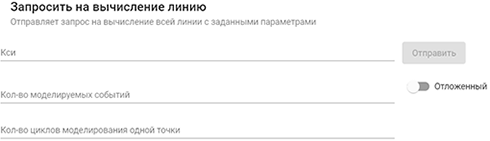
\includegraphics[width=\textwidth]{figures/request-line.png}
	\caption{Панель старта расчета линии значений}
	\label{fig:request-line}
\end{figure}

После выставления нужных пользователю параметров, необходимо нажать кнопку <<Отправить>> после чего данные отправляются на сервер и результат будет перерисован на интерфейсе приложения. Результаты вычислений будут добавлены на основной график в реальном времене, поэтому пользователю не нужно обновлять страницу с графиком.

Как только запрос был отправлен на сервер создается \textit{websocket} соединение между \textit{web}-браузером пользователя и серверным приложением, тем самым подписывая клиента на получение денных от сервера, как только они будут готовы.

На графике кросс-секции $\sigma \times Br({Z}^{\prime} \rightarrow {W}^{+}{W}^{-})$ для ${Z}^{\prime}_{SSM}$ прорисовывается линия с новыми значениями в то время, как серверное приложение начинает параллельно для нескольких значений массы ${M}_{{Z}^{\prime}}$ моделировать столкновение протонов.

Так как в реальном столкновении протонов рождается очень большое количество различных частиц то моделирование такой задачи при помощи генератора \textit{PYTHIA} требует значительных ресурсов центрального процессора сервера и занимает продолжительное время. Приложение созданное в рамках данной работы имеет \textit{web}-интерфейс, что позволяет сразу нескольким пользователям работать в нем и отправлять запросы на вычисления. В связи с этим вводится ограничение на количество параллельно запущенных процессов моделирования для каждого пользователя.

Под панелью для запроса вычислений располагается список ранее отправленных запросов, как показано на рисунке~\ref{fig:preferences}. Нажав на крестик <<X>> можно удалить линию на графике.

Все запросы на вычисление сохраняются для конкретного пользователя и загружаются из локального хранилища данных при обновлении страницы.

\begin{figure}[!h]
	\centering
	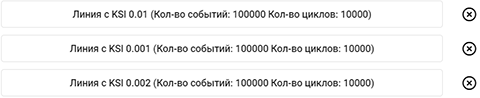
\includegraphics[width=\textwidth]{figures/preferences.png}
	\caption{Список отображаемых линий}
	\label{fig:preferences}
\end{figure}

Как видно из рисунка~\ref{fig:offline-calc} у пользователя есть возможно отправить <<Отложенный>> запрос на вычисление для удобства вычисления линий. Отложенный запрос означает, что запрос добавиться в очередь вычисления на стороне сервера. Запрос будет сохраняться до того момента пока вычислительные ресурсы не освободятся и только после этого запрос обработается и начнется процесс имитационного моделирования.

\begin{figure}[!h]
	\centering
	
\includegraphics[width=0.4\textwidth]{figures/offline-calc.png}
	\caption{Переключатель в <<отложенный>> режим отправки запросов}
	\label{fig:offline-calc}
\end{figure}

Даже самая простая задача расчета модели занимает большое время. К примеру запрос пользователя расчитать линию для всех значений ${M}_{{Z}^{\prime}}$, а в рамках данного проекта это пять тысяч точек на графике от 0 до 5000 ГэВ, и количеством генерируемых событий займет 9,7 часа. 

В таком простом случае полученное значение будет подвержено значительной статистической ошибки. Чтобы убрать данную статистическую ошибку требуются дополнительные циклы имитационного моделирования, что увеличивает затраченное время в разы. 

Так как вычисления могут занять довольно много времени то вычисляются не все значения массы ${M}_{{Z}^{\prime}}$. Устанавливается шаг для вычислений к примеру 100 ГэВ и в качестве входного значения массы подставляются значения в 100 ГэВ, 200 ГэВ и т.д. Этот подход экономит значительное количество ресурсов вычислительной машины и экономит время для получения общей картины поведения распределения ограничений на угол смешивания. Дополнительно на стороне сервера предусмотрено хранение уже рассчитаные результатов по выходным данным имитационного моделирования.


Предусмотрена возможность отправлять запросы на вычисление только одной точки на графике. Данная возможно позволяет узнать точное значение кросс-секции $\sigma \times Br({Z}^{\prime} \rightarrow {W}^{+}{W}^{-})$ для конкретной массы ${Z}^{\prime}_{SSM}$-бозона и не тратить время на вычисления значений всех масс ${M}_{{Z}^{\prime}}$ для заданной $\xi$. Панель позволяющая отправлять такие запросы представлена на картинке~\ref{fig:request-point}.

\vspace{16pt}
\begin{figure}[!h]
	\centering
	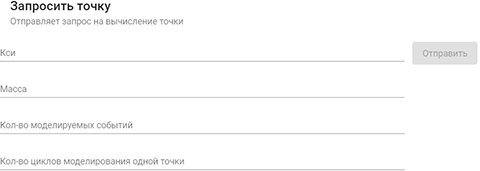
\includegraphics[width=\textwidth]{figures/request-point.png}
	\caption{Панель старта расчета одного значения}
	\label{fig:request-point}
\end{figure}

Общий процесс вычисления всех значений для масс ${M}_{{Z}^{\prime}}$ отображается в виде прогресс бара в самом низу веб страницы. Как показано на рисунке~\ref{fig:progress} данный элемент не имеет каких-либо точек взаимодействия с пользователем и несет лишь информативный характер.

Компонент <<Прогресс вычислений>> содержит комплексную информацию о ходе вычислений: количество вычисляемых значений в данный момент времени, лимит вычисляемых точек в одно время для сессии одного пользователя, очередь запросов от пользователя и количество успешно полученных результатов.

Так как вычисления могут занять довольно много времени то вычисляются только текущие запросы для текущей сессии пользователя. К примеру если, лимит на вычисления равен десять запросов в одно время и пользователь запустил процесс вычисления целой линии значений, а после закрыл страницу \textit{web}-приложения то будут произведены вычисления только этих десяти значений. Дальнейшие вычисления будут возобновлены, когда пользователь вновь откроет страницу \textit{web}-интерфейса или другой пользователь отправить запрос на вычисление с теми же входными параметрами.

\begin{figure}[!h]
	\centering
	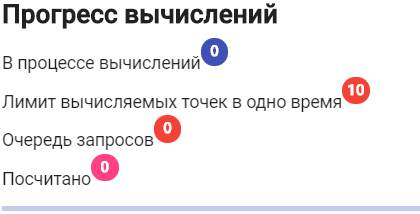
\includegraphics[width=0.5\textwidth]{figures/progress.png}
	\caption{Прогресс вычислений}
	\label{fig:progress}
\end{figure}

Интерфейс результатов и вычислений выполнен в виде \textit{SVG} элемента и состоит из графика кросс-секции $\sigma \times Br({Z}^{\prime} \rightarrow {W}^{+}{W}^{-})$ для масс ${M}_{{Z}^{\prime}}$ (рисунок~\ref{fig:graph-1}).

\begin{figure}[!h]
	\centering
	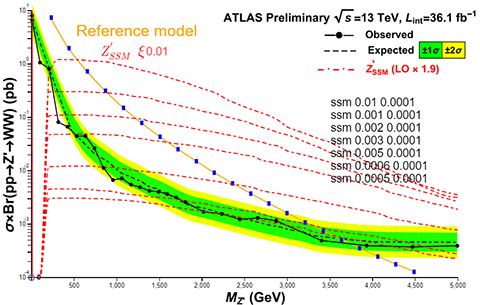
\includegraphics[width=\textwidth]{figures/graph-1.png}
	\caption{Панель старта расчета линии значений}
	\label{fig:graph-1}
\end{figure}

На графике отображены статические элементы полученные из математических формул и вычислений, а также данные не вычисляемые в рамках данной диссертации и полученные от коллаборации \textit{ATLAS}, такие  как \textit{reference model}, \textit{observed} значения, \textit{expected} значения с областью в два стандартных отклонения~\cite{2part-pankov}.

Представленный на рисунке~\ref{fig:graph-1} график имеет элемент управления - вертикальная красная линия. Данная линия добавлена, чтобы помочь пользователю определить занчение кросс-секции для массы ${M}_{{Z}^{\prime}}$ и выбранным углом смешивания $\xi$. Близлежащие значения к данной вертикальной линии будут подсвечены на графике и их точное значение всегда отображается в правой части графика.

Перейдя на вкладку <<Результат>> из меню приложения (рисунок~\ref{fig:menu}) пользователю будет предоставлен результат работы приложения, который показан на рисунке~\ref{fig:graph-result}.

\begin{figure}[!h]
	\centering
	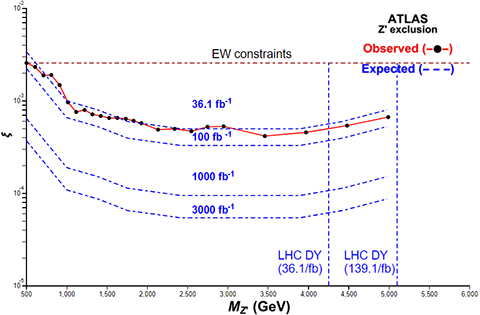
\includegraphics[width=\textwidth]{figures/graph-result.png}
	\caption{Ограничения на угол смешивания $Z$-${Z}^{\prime}$ полученные из обработки данных имитационного моделирования}
	\label{fig:graph-result}
\end{figure}

Результат представляет собой график зависимости угла смешивания $\xi$ и массы ${M}_{{Z}^{\prime}}$ и отражает ограничения на угол смешивания ${Z}^{\prime}$-бозонов в модели \textit{SSM}. 

Значениями ломаной \textit{Observed} являются точки ($\xi$) пересечения моделируемых линий и кривой \textit{expected}, которые отображены на рисунке~\ref{fig:graph-1}. В данной диссертационной работе при помощи разработанной имитационной модели рождения $Z^\prime$ - бозонов в протон-протонных столкновениях с учетом эффектов $Z$ - $Z^\prime$ смешивания были получены ограничение на угол смешивания ${Z}^{\prime}$-бозонов для до светимости 3000 фб${}^{−1}$ и равняется $6\times{10}^{-5}$.


\begin{figure}[!h]
	\centering
	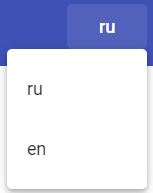
\includegraphics[width=0.2\textwidth]{figures/language-switch.png}
	\caption{Смена языка \textit{web}-страницы}
	\label{fig:language-switch}
\end{figure}

Каждая веб страница имеет функционал для смены отображаемого языка. Данный функционал добавлен в правом верхнем углу \textit{web}-интерфейса, рисунок~\ref{fig:language-switch}.

Исходя из того, что большая часть использованной литературы при исследовании проблемы описанной в данной диссертационной работе является англоязычной было принято решение реализовать возможность смены языка на котором отображается текст приложения.

